\documentclass[a4paper]{article}
\usepackage[a4paper,  margin=1.0in]{geometry}

\usepackage{graphicx}
\usepackage{float}
\usepackage{hyperref}
\usepackage{listings}
\lstset{
basicstyle=\small\ttfamily,
columns=flexible,
breaklines=true
}

\usepackage{polski}
\usepackage[utf8]{inputenc}
\begin{document}


\title{Ćwiczenie nr 4 z MBI, Analiza danych sekwencyjnych człowieka}
\author{Mateusz Chydziński, Michał Sypetkowski}
\maketitle

\section{Ogólne informacje}
Repozytorium git: \url{https://github.com/msypetkowski/MBI-exercises.git}.
W katalogu \texttt{cw4} repozytorim zawiera skrypty/polecenia użyte do przeprowadzenia eksperymentów.


\section{Liczenie pokrycia}
Największa mediana pokrycia została zarejestrowana dla próbki \texttt{NA19137} i wynosi \texttt{76.03475}. Najmniejsza wyliczona
mediana charakteryzuje próbkę o numerze \texttt{NA18991} a jej wartość to \texttt{21.06271}.


\section{Wykrywanie zmian liczby kopii DNA przy użyciu narzędzia CODEX}
Statystyki kontroli jakości:
\begin{verbatim}
Excluded 279 exons due to extreme coverage.
Excluded 18 exons due to extreme exonic length.
Excluded 22 exons due to extreme mappability.
Excluded 15 exons due to extreme GC content.
After taking union, excluded 318 out of 4702 exons in QC.
\end{verbatim}
Zgodnie z powyższymi zapisami logów narzędzia CODEX, zostało usuniętych \texttt{318} eksonów w \texttt{wyniku kontroli jakości}.
Po zmianie parametrów progowych \texttt{gc\_thresh\_from, gc\_thresh\_to)} na wartości \texttt{30, 70} statystki prezentują się następująco:

\begin{verbatim}
Excluded 279 exons due to extreme coverage.
Excluded 18 exons due to extreme exonic length.
Excluded 22 exons due to extreme mappability.
Excluded 324 exons due to extreme GC content.
After taking union, excluded 472 out of 4702 exons in QC.
\end{verbatim}
Zmieniła się zatem liczba wykluczonych eksonów - wykluczono \texttt{472}.

Wykryto \texttt{438 zmian liczby kopii}. Wśród nich jest \texttt{264 duplikacji} i \texttt{174 delecji}.
Występują \texttt{3 homozygotyczne delecje} (copy\_no == 0) dla próbek \texttt{NA18486, NA18912 oraz NA18965}:
\begin{verbatim}

  sample_name chr cnv    st_bp    ed_bp length_kb st_exon ed_exon raw_cov norm_cov copy_no lratio    mBIC targetCount
X.147     NA18486  20 del 56793551 56803479     9.929    3653    3655       0       21       0     21   0.677           2
X.339     NA18912  20 del 56793551 56803479     9.929    3653    3655       0       21       0     21   0.677           2
X.361     NA18965  20 del 61460052 61460361      0.31    4036    4037       0       24       0     24 320.948           1
\end{verbatim}

\begin{figure}[h]
    \centering
    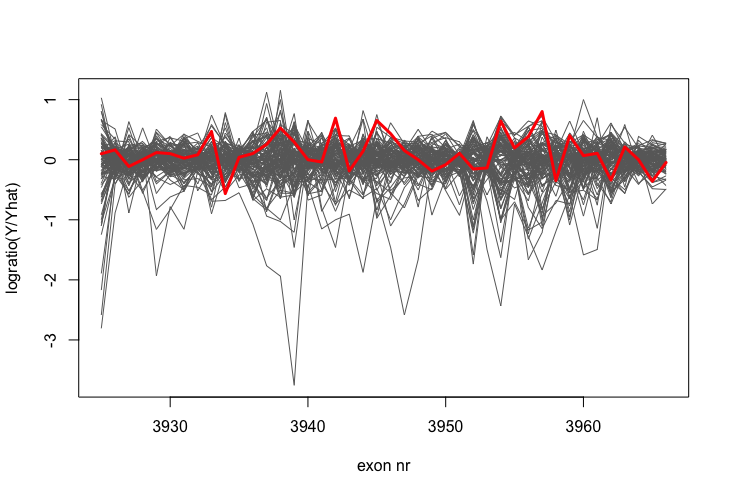
\includegraphics[width=1.0\textwidth]{plot_change_no_1.png}
    \label{fig:igv}
    \caption[]{Wykres dla zmiany numer 1}
\end{figure}

\section{Wnioski}


\end{document}
